% !TeX spellcheck = en_GB
\documentclass[answers]{exam}
% addpoints

\ifprintanswers
	\usepackage[type1]{libertine}
	\usepackage[a4paper]{geometry}
	\usepackage{parskip}
\else
\fi

\usepackage{tikz}
	\usetikzlibrary{arrows}
\usepackage{circuitikz}

\usepackage{amsmath, amsthm, amssymb} 
\usepackage{tabularx}
\usepackage[english]{babel}
\usepackage{enumitem}
\usepackage{gensymb}
\usepackage{bm}
\usepackage{graphicx}
\usepackage{xcolor}
\usepackage{float}
\usepackage{wrapfig}
\usepackage[makeroom]{cancel}
\usepackage{multicol}
\usepackage{vwcol} 	 % Provides variable multicol
\usepackage{commath} % Provides good differentials
\usepackage{siunitx} % Provides good units
\usepackage{nicefrac}
\usepackage{dashrule}

\usepackage[titletoc,title,toc,page]{appendix}
\usepackage{hyperref}
\hypersetup{
	pdftitle={SJPO Training -- Ciruclar \& Angular Motion Problem Set},
	pdfauthor={Sun Yudong, Tan Jing Long},
	bookmarksnumbered=true,
	bookmarksopen=true,
	bookmarksopenlevel=2,
	pdfstartview=Fit,
	pdfpagemode=UseOutlines,
	colorlinks=true,
	linkcolor=black,
	filecolor=magenta,      
	urlcolor=blue
}

\newcommand{\uvec}[1]{\boldsymbol{\hat{\textbf{#1}}}}
\def\doubleunderline#1{\underline{\underline{#1}}}

\renewcommand{\ttdefault}{cmtt}

\newenvironment{multicolFigure}
{\par\medskip\noindent\minipage{\linewidth}}
{\endminipage\par\medskip}

\ifprintanswers
	\title{\vspace{-1cm} SJPO Training\\ Circular \& Angular Motion Problem Set}
	\author{Worked Solutions by Sun Yudong \\ {\small Questions originally compiled by Tan Jing Long on May 7, 2016}}
	\date{May 3, 2018}
\else
	\title{SJPO Training\\ Circular \& Angular Motion Problem Set}
	\author{Tan Jing Long\\
		Hwa Chong Institution}
	\date{May 7, 2016}
\fi

\begin{document}
\maketitle

\section{General Round}
\subsection{Centripetal Force}
\begin{questions}

\question{A particle moves at a constant speed in a circular path with a radius of \(\SI{2.06}{\centi\meter}\). If the particle makes four revolutions each second, what is the magnitude of its acceleration?
\begin{solutionorbox}[60mm] \(\SI{13}{\meter/\second\squared}\) 
	\begin{align*}
		\omega &= 4 \times 2\pi = 8\pi \\
		a_c &= r\omega^2 = \left(2.06\times 10^{-2}\right)\left(8\pi\right)^2 \\
		&= \SI{13}{\meter/\second\squared}
	\end{align*}
\end{solutionorbox}
}

\ifprintanswers
	\vfill
\fi

\question{A carnival Ferris wheel has a \(\SI{15}{\meter}\) radius and completes five turns about its horizontal axis every minute. What is the acceleration of the passenger at his lowest point during the ride?
\begin{solutionorbox}[60mm] \(\SI{4.1}{\meter/\second^2}\), taking upwards as positive. 
	\begin{align*}
		\omega &= 2\pi \times \frac{5}{60} = \frac{\pi}{6} \\
		a_c &= r\omega^2 = \left(15\right)\left(\frac{\pi}{6}\right)^2 \\
		&= \SI{4.1}{\meter/\second^2}
	\end{align*}
	As this is a Ferris wheel and the angular velocity is constant, the magnitude of the acceleration experienced by the passenger will also be constant.
\end{solutionorbox}
}

\ifprintanswers
	\vfill
	\pagebreak
\fi

\question{A tether ball is on a \(\SI{2.1}{\meter}\) string which makes an angle of \(\SI{22}{\degree}\) with the vertical as it moves around the pole in a horizontal plane. If the mass of the ball is \(\SI{1.3}{\kilogram}\), what is the ball's speed?
\begin{solutionorbox}[40mm] \(\SI{1.8}{\meter/\second}\)
		
	\begin{minipage}{3cm} 
		\hspace{0.7cm}
		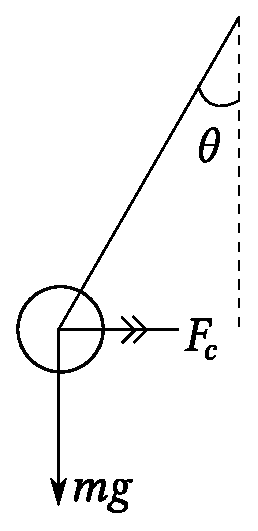
\includegraphics[width=1.5cm]{tetherball.eps}
	\end{minipage}
	\begin{minipage}{\linewidth - 3cm}
	Since the ball does not have any acceleration in the vertical direction:
		\begin{align*}
			T=\frac{mg}{\cos\theta} \implies F_c &= T\sin\theta = mg\tan\theta \\
			a_c &=g\tan\theta=\frac{v^2}{r} \\
			v &= \sqrt{rg\tan\theta} \\
			&= \sqrt{\left(l\sin\theta\right)g\tan\theta} = \SI{1.77}{\meter\per\second}
		\end{align*}
	\end{minipage}
\end{solutionorbox}
}

\ifprintanswers
	\vfill
	\section*{Important Concept}
	\vspace{-0.5cm}
	\hdashrule{0.95\textwidth}{0.1mm}{1pt}
	\vspace{-0.5cm}
	\subsection*{Rolling without Slipping}
	
	The motion of a rolling wheel is the sum of the translational motion of the center of mass plus the rotational motion of the wheel around the center of mass:
	
	\begin{figure}[h]
		\centering
		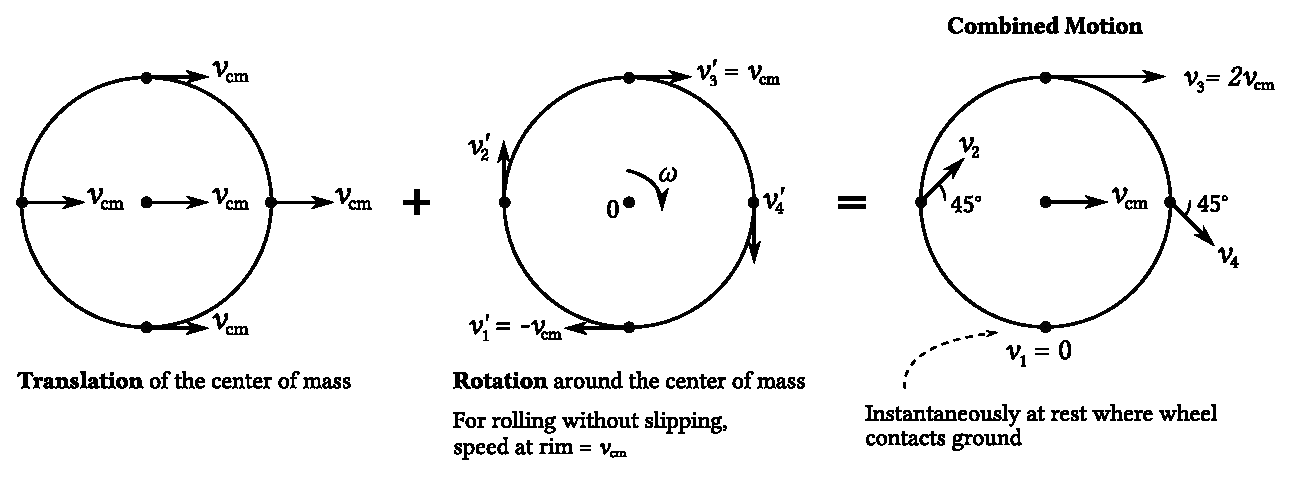
\includegraphics[width=0.9\linewidth]{rollingwithoutslipping.eps}
		\caption{Rolling without slipping illustration}
		\label{fig:rollingwithoutslipping}
	\end{figure}
	\vspace{-0.5cm}
	\hdashrule{0.95\textwidth}{0.1mm}{1pt}
	\vfill
	\pagebreak
\fi

\question{A tractor moving forward at uniform speed on horizontal ground has a front wheel diameter of \(\SI{0.8}{\meter}\) and back wheel diameter of \(\SI{1.25}{\meter}\). The horizontal distance between the axles of the two wheels is \(\SI{2}{\meter}\). During a trip a pebble stuck to the front wheel flew off the wheel at the highest point. \(\SI{0.2}{\second}\) later, another pebble flew off the back wheel at its highest point too. The two pebbles landed on the same spot on the ground. Find the speed of the tractor.
\begin{solutionorbox}[40mm] \(\SI{5}{\meter/\second}\) 
	
	\vspace{-0.5cm}
	\begin{minipage}{5.5cm} 
		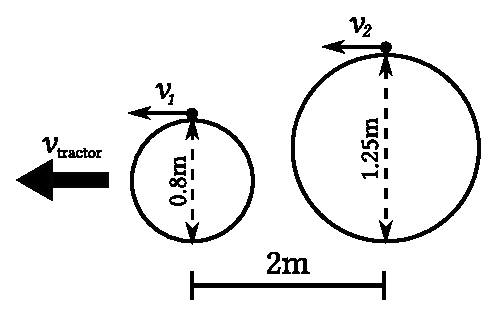
\includegraphics[width=5cm]{tractor.eps}
	\end{minipage}
	\begin{minipage}{\linewidth - 5.5cm}
		\begin{align}
		S_y&=\frac{1}{2}at^2 \implies t=\sqrt{\frac{2S_y}{g}} \\
		\implies S_{x_i}&=v_it = v_i\sqrt{\frac{2S_{y_i}}{g}}\\
		v_1&=v_2 = 2v_{\text{tractor}}
		\end{align}
	\end{minipage}

	We can take wheel 1 as the origin, then with the above 3 equations:
	\begin{align*}
		S_1 &= S_2 \\
		\sqrt{\frac{2S_{y_1}}{g}}\left(2v_{\text{tractor}}\right) &= -2 +  0.2v_{\text{tractor}} + \sqrt{\frac{2S_{y_2}}{g}}\left(2v_{\text{tractor}}\right) \\
		v_{\text{tractor}}\left[2\sqrt{\frac{2(0.8)}{g}} - 2\sqrt{\frac{2(1.25)}{g}} -0.2 \right] &= -2 \\
		v_{\text{tractor}} &= \SI{4.98}{\meter\per\second}
	\end{align*}
	
\end{solutionorbox}
}

\end{questions}

\subsection{Position-dependent Quantities}
\begin{questions}

\question{A large spool of rope lies on the ground, as shown in the diagram below. The end, labelled \(X\), is pulled a distance \(S\) in the horizontal direction. The spool rolls without slipping. In terms of \(S\), determine the distance the spool's center of mass moves.
\begin{center}
\begin{tikzpicture}
\draw (0,1) circle (1);
\draw (-1.5,0) -- (2.5,0);
\draw (0,2) -- (1.5,2);
\node at (1,2.2) {X};
\end{tikzpicture}
\end{center}
\begin{solutionorbox}[40mm] \(S/2\) 
	
	The solution is fairly straightforward: we basically want to find what is the distance travelled by the center of mass, given that the top point travels a distance $S$. 
	
	Referring to Figure \ref{fig:rollingwithoutslipping} on the previous page, we need only integrate all the velocity to obtain the distance $S$ travelled --- if the center of mass travels a distance $D$, the top point travels $2D$. Thus, if the top point ($X$) travels $S$, the center of mass will travel $S/2$.

\end{solutionorbox}
}

\question{\(PQRS\) is a light, rigid rod with masses attached to it as shown in the diagram, where \(PQ = QR = RS = l\). Determine the moment of inertia of the system about \(XY\).
\begin{center}
\begin{tikzpicture}
\draw [dashed] (0,1) -- (0,-1);
\node at (0.3,1) {\(X\)};
\node at (0.3,-1) {\(Y\)};

\draw (0,0) -- (-3,0);
\fill (0,0) circle (1mm);
\node at (-0.25,0.3) {\(S\)};
\fill (-1,0) circle (1mm);
\node at (-1,0.3) {\(R\)};
\fill (-2,0) circle (1mm);
\node at (-2,0.3) {\(Q\)};
\fill (-3,0) circle (1mm);
\node at (-3,0.3) {\(P\)};
\end{tikzpicture}
\end{center}
\begin{solutionorbox}[35mm] \(14ml^2\) 
	\begin{align*}
		\sum_{i}^{}m_ir_i^2 &= m(3l)^2 + m(2l)^2 + m(l)^2 + m(0)^2\\
		&= 14ml^2
	\end{align*}	
	\textit{Question modified from original \texttt{[SJPO 2008/G15]}, in which $P=4m$, $Q=3m$, ... }
\end{solutionorbox}
}

\question{Two identical rectangular bricks of length \(S\) are piled with one on top of the other on a table. What is the maximum distance \(L\) (see the figure below) that the top brick can be extended beyond the edge of the table for the system to remain balanced? (Note that the figure is not drawn to scale.)
\begin{figure}[h]
\begin{center}
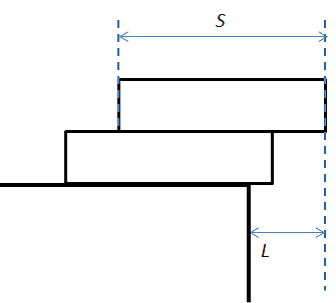
\includegraphics[scale=0.4, clip=false, trim=0 50 0 25]{mcq_2012_22}
\end{center}
\end{figure}
\begin{solutionorbox}[35mm] $\nicefrac{3}{4}\ S$
	
	Starting from the top down, we place every brick above the one below at its center of mass. For the first layer, it's rather straightforward:
	\begin{center}
		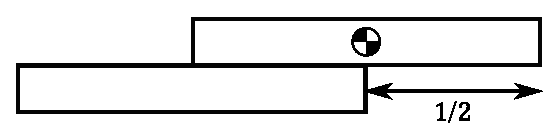
\includegraphics[width=5cm]{stacking-firstlayer.eps}
	\end{center}
	Now we find the new center of mass of this system. Taking moments about the right edge of the top block:
	\vspace{-0.5cm}
	\begin{align*}
		2\cancel{m}\left(x_{cm}\right) &= \cancel{m}\left(\frac{1}{2}S\right) + \cancel{m}\left(S\right) \\
		x_{cm} &= \left(\frac{3}{2} \div 2\right)S\\
		&=\frac{3}{4}S
	\end{align*}
	Since we only have 2 blocks, our working ends here. For more blocks, we continue to find the subsequent center of masses. By putting the center of mass of the system at the edge, we achieve the maximum $L$ is thus $\nicefrac{3}{4}\ S$.
\end{solutionorbox}
}

\ifprintanswers
	\pagebreak
\fi
\question{A diatomic molecule consists of two point masses, \(m_1\) and \(m_2\), separated by a distance \(r\). If \(x\) is the distance from \(m_1\) to the center of mass, what is the moment of inertia about an axis parallel to the molecular axis and passes through the center of mass. Note that the molecular axis is the line joining the two atoms in the diatomic molecule.
\begin{solutionorbox}[35mm] 0 
	
	The center of mass of the system must lie along the molecular axis, hence we are finding $I$ about the molecular axis. Since the point masses are of a distance $0$ away from the axis, 
	\begin{equation*}
		I=\sum_{i}m_ir_i^2=\sum_{i}m_i(0)^2=0
	\end{equation*}
\end{solutionorbox}
}

\ifprintanswers
	\vfill
\fi


\question{In the figure below, a \(\SI{24}{\centi\meter}\) length of uniform wire, is bent into a right-angled triangle. The two shorter sides lies on the \(x\) and \(y\) axes as shown below. You may neglect the thickness of the wire. Determine the \(x\)- and \(y\)-coordinates of the centre of mass, in cm.
\begin{figure}[h]
\begin{center}
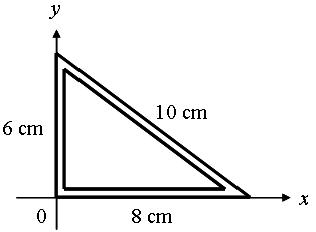
\includegraphics[scale=0.55, clip=false, trim=0 40 0 10]{mcq_2010_25}
\end{center}
\end{figure}

\ifprintanswers
	\vspace{0.5cm}
\fi

\begin{solutionorbox}[60mm] (3.0,2.0) 
	
	Let the center of mass be at $(x,y)$, and the density of the wire be $\sigma$
	
	Taking moments about the $y$-axis:
		\begin{align*}
			24\sigma x&=8\sigma\left(\frac{8}{2}\right) + 10\sigma\left(\frac{5}{10}\times 8\right) &&\text{\textit{(Similiar Triangles)}} \\
			24x&=32+40 \\
			&=72 \\
			x &= 3
		\end{align*}
	Taking moments about the $y$-axis:
		\begin{align*}
			24\sigma y&=6\sigma\left(\frac{6}{2}\right) + 10\sigma\left(\frac{5}{10}\times 6\right) &&\text{\textit{(Similiar Triangles)}} \\
			24x&=18+30 \\
			&=48 \\
			y &= 2
		\end{align*}
	Thus, the center of mass is $(3.0,2.0)$.
\end{solutionorbox}
}

\end{questions}

\ifprintanswers
	\pagebreak
\fi
\subsection{Rigid Body Mechanics}
\begin{questions}

\question{A drum has a radius of \(\SI{0.40}{\meter}\) and a moment of inertia of \(\SI{4.5}{\kilogram\meter^2}\). The frictional torque of the drum axle is \(\SI{3.0}{\newton\meter}\). A \(\SI{15}{\meter}\) length of rope is wound around the rim. The drum is initially at rest. A constant force is applied to the free end of the rope until the rope is completely unwound and slips off. At that instant, the angular velocity of the drum is \(\SI{13}{\radian/\second}\). The drum then decelerates and comes to a halt. Determine the constant force applied to the rope.
	\begin{solutionorbox}[75mm] $\SI{33}{\newton}$
		
			We make use of rotational analogues of kinematic equations.
			\begin{multicols}{2}
				\noindent
				\begin{align*}
					\omega_f^2 &= \cancelto{0}{\omega_i^2}+2\alpha\theta \\
					\alpha &= \frac{\omega_f^2}{2\theta} \\
					&= \frac{\omega_f^2}{2\left(\frac{L}{\cancel{2\pi} r}\cdot \cancel{2\pi}\right)} \\
					&= \frac{169}{75}
				\end{align*}
				\begin{align*}
					\sum \tau = \tau_{\text{rope}} - \tau_{f} &= I\alpha \\
					\tau_{\text{rope}} &= I\alpha + \tau_{f} \\
					&= 13.14 \\\\
					\because \tau_{\text{rope}} &= F_{\text{rope}}\times r \\
					\therefore F_{\text{rope}} &= \frac{13.14}{0.40} = \SI{32.85}{\newton}
				\end{align*}
			\end{multicols}
	\end{solutionorbox}
}

\end{questions}

\ifprintanswers
\else
	\pagebreak
\fi
\section{Special Round}

\begin{questions}

\question[8]{A daredevil astronomer stands at the top of his observatory dome wearing roller skates and starts with negligible velocity to coast down over the dome surface.
\begin{figure}[h]
\begin{center}
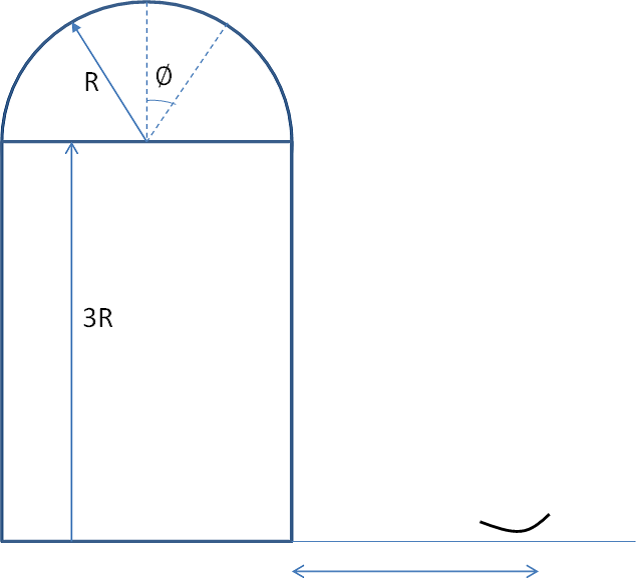
\includegraphics[scale=0.4, clip=false, trim=0 40 0 0]{2011_2}
\end{center}
\end{figure}
\begin{enumerate}
	\item{Neglecting friction, at what angle \(\phi\) does he leave the dome's surface?}
	\item{If he were to start with an initial velocity \(v_0\), at what angle \(\phi\) would he leave the dome?}
	\item{For the observatory shown above, how far from the base should his assistant position a net to break his fall, as in the situation in 1? Evaluate your answer for \(R = \SI{8.0}{\meter}\).}
\end{enumerate}
\begin{solutionorbox}[115mm] $\phi = \SI{48.2}{\degree}; \cos{\phi} = \frac{2gR+v_0^2}{3gR}; \SI{7.4}{\meter}$
	
	We take the daredevil as a point mass.
	\begin{enumerate}[label={[\arabic*]}]
		\item {\color{white} .}\vspace{-0.5cm}
		
			\begin{minipage}{3cm} 
				\hspace{0.7cm}
				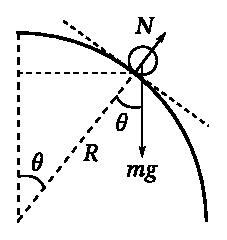
\includegraphics[width=2.5cm]{daredevil.eps}
			\end{minipage}
			\begin{minipage}{\linewidth - 3cm}
				By Conservation of Energy,
				\vspace{-0.3cm}
				\begin{align*}
				\text{GPE} = mgh &= \frac{1}{2}mv^2 = \text{KE} \\
				mg\left[R\left(1-\cos\theta\right)\right] &= \frac{1}{2}mv^2 \\
				v^2 &= 2gR\left(1-\cos\theta\right)
				\end{align*}
			\end{minipage}
		
			Analysing the forces on the mass,
			%\vspace{-0.3cm}
			\begin{align*}
				\sum F = mg\cos\theta - N &= F_c = ma_c \\
				&= m\left[\frac{v^2}{R}\right]
			\end{align*}
			When the daredevil leaves the dome at $\theta = \phi$, $N = 0$,
			%\vspace{-0.3cm}
			\begin{align*}
			 \cancel{m}g\cos\phi &= \cancel{m}\left[\frac{v^2}{R}\right] \\
			 \cancel{g}\cos\phi &= \frac{2\cancel{g}\cancel{R}\left(1-\cos\phi\right)}{\cancel{R}} \\
			 3\cos\phi &= 2 &\implies \phi = \arccos\frac{2}{3} = \doubleunderline{48.2\degree}
			\end{align*}
		\item We apply conservation of energy again
			\begin{align*}
				\frac{1}{2}\cancel{m}v_0^2 + \cancel{m}gh &= \frac{1}{2}\cancel{m}v_1^2 \\
				v_0^2 + 2g\left[R\left(1-\cos\theta\right)\right] &= v_1^2
			\end{align*}
			Substituting into the second part of the part [1]:
			\begin{align*}
				g\cos\phi &= \frac{v_0^2 + 2gR\left(1-\cos\phi\right)}{R} \\
				gR\cos\phi + 2gR\cos\phi &= v_0^2 + 2gR \\
				\cos\phi &= \frac{v_0^2 + 2gR}{3gR} &\implies \phi = \arccos \left(\frac{v_0^2 + 2gR}{3gR}\right)
			\end{align*}
		\item {\color{white} .}\vspace{-0.5cm}
		
			\begin{minipage}{3cm} 
				\hspace{0.7cm}
				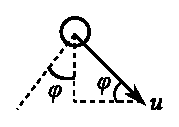
\includegraphics[width=2.5cm]{daredevil2.eps}
			\end{minipage}
			\begin{minipage}{\linewidth - 3cm}
				Using 2D kinematics, taking down and right as positive:
				\begin{align*}
				S_y = R\left(3 + \cos\phi\right) &= u_yt + \frac{1}{2} at^2 \\ 
				&= u\left(\sin\phi\right)t + \frac{1}{2} gt^2 \\
				&= \sqrt{2gR\left(1-\cos\phi\right)}\left(\sin\phi\right)t + \frac{1}{2} gt^2 \\
				\implies t &= 1.95689 \text{~~or~~} \cancel{-3.05603}
				\end{align*}
			\end{minipage}
			From $t$, we obtain the distance $S_x$ from the point that he leaves the dome:
			\begin{align*}
				S_x &= u\cos\phi \times t \\
				&= \sqrt{2gR\left(1-\cos\phi\right)}\left(\cos\phi\right)t
			\end{align*}
			The base should then be placed at distance $D$ away:
			\begin{align*}
				D &= S_x - R(1-\sin\phi) \\
				&= \sqrt{2gR\left(1-\cos\phi\right)}\left(\cos\phi\right)t - R(1-\sin\phi) \\
				&= \doubleunderline{\SI{7.4}{\meter}}
			\end{align*}
	\end{enumerate}
\end{solutionorbox}
}

\end{questions}

\end{document}